% Created by tikzDevice version 0.12.6 on 2025-09-19 11:10:47
% !TEX encoding = UTF-8 Unicode
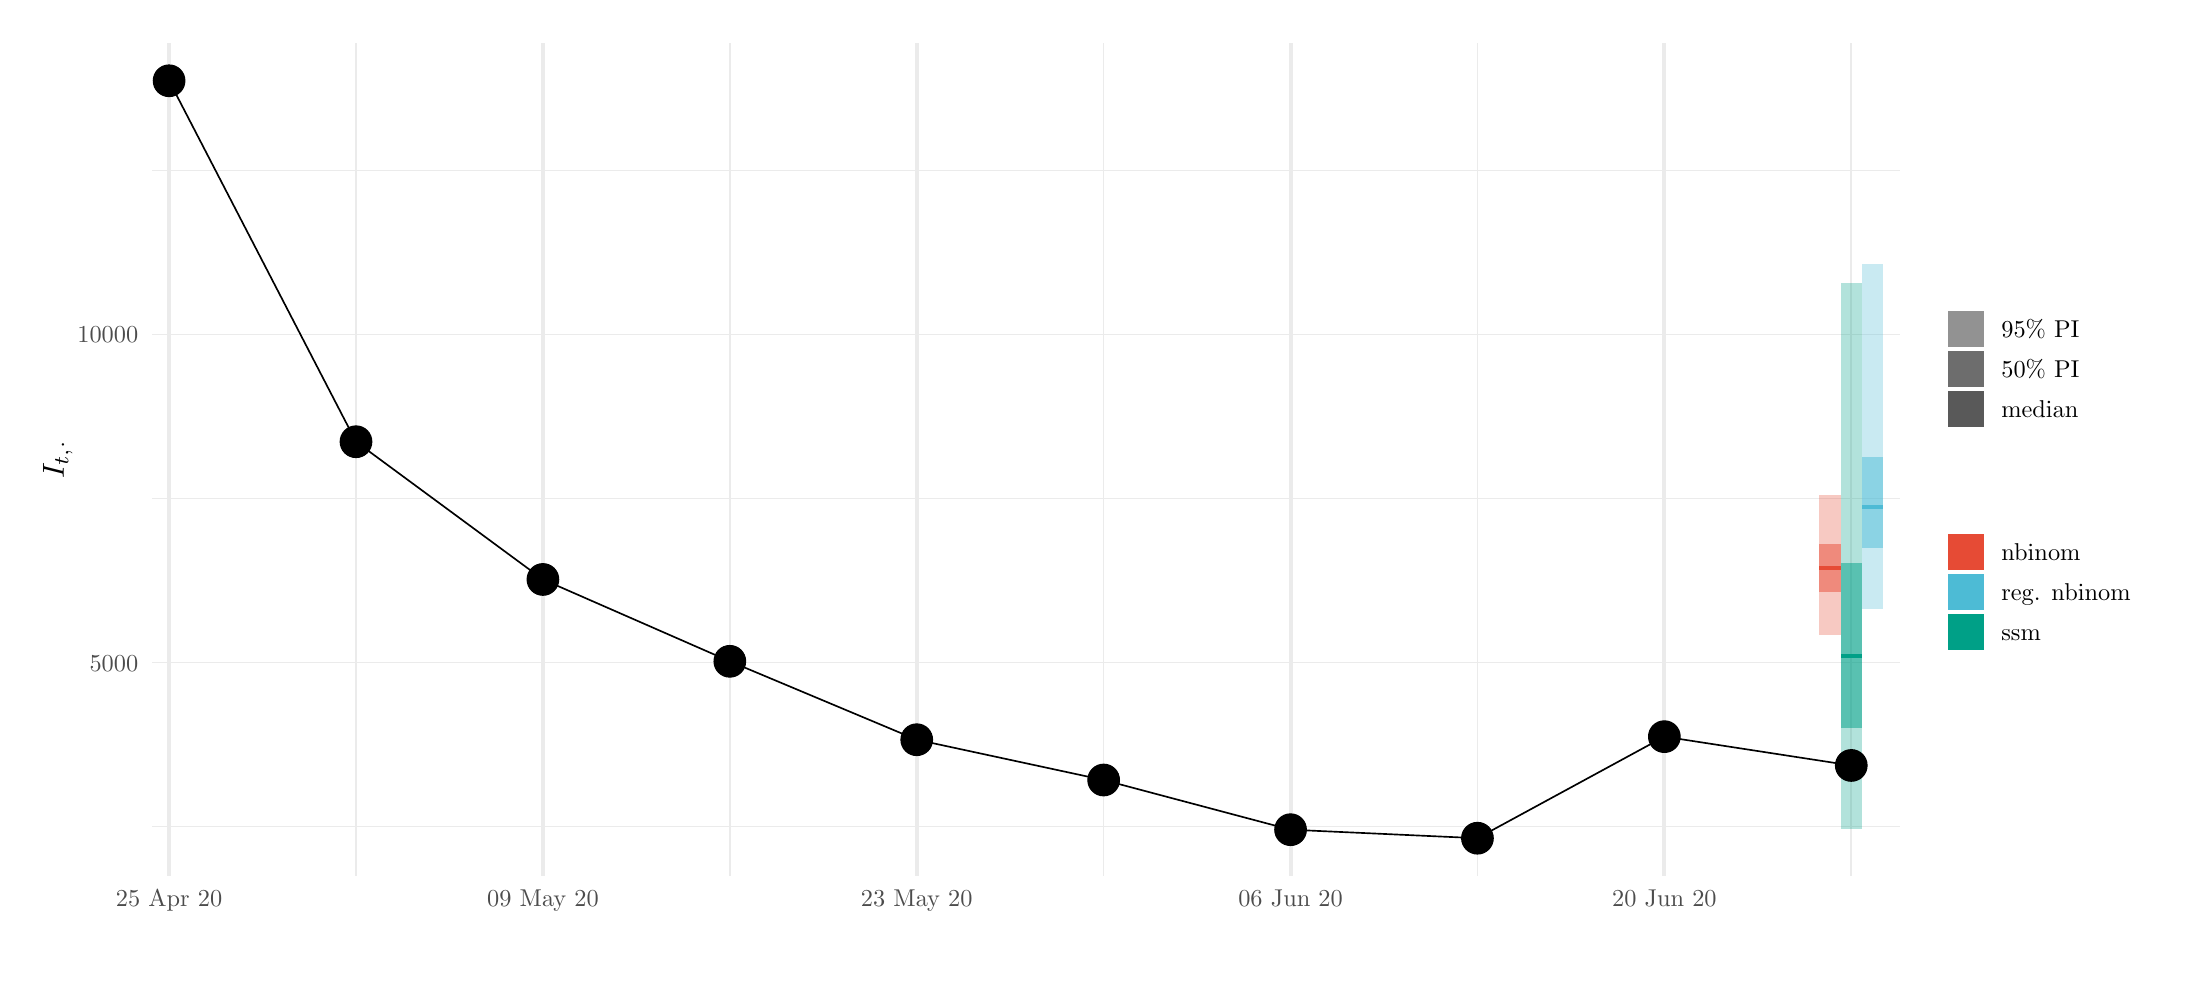
\begin{tikzpicture}[x=1pt,y=1pt]
\definecolor{fillColor}{RGB}{255,255,255}
\path[use as bounding box,fill=fillColor,fill opacity=0.00] (0,0) rectangle (770.88,337.26);
\begin{scope}
\path[clip] ( 44.91, 30.69) rectangle (676.72,331.76);
\definecolor{drawColor}{gray}{0.92}

\path[draw=drawColor,line width= 0.3pt,line join=round] ( 44.91, 48.54) --
	(676.72, 48.54);

\path[draw=drawColor,line width= 0.3pt,line join=round] ( 44.91,167.08) --
	(676.72,167.08);

\path[draw=drawColor,line width= 0.3pt,line join=round] ( 44.91,285.62) --
	(676.72,285.62);

\path[draw=drawColor,line width= 0.6pt,line join=round] (118.64, 30.69) --
	(118.64,331.76);

\path[draw=drawColor,line width= 0.6pt,line join=round] (253.72, 30.69) --
	(253.72,331.76);

\path[draw=drawColor,line width= 0.6pt,line join=round] (388.80, 30.69) --
	(388.80,331.76);

\path[draw=drawColor,line width= 0.6pt,line join=round] (523.87, 30.69) --
	(523.87,331.76);

\path[draw=drawColor,line width= 0.6pt,line join=round] (658.95, 30.69) --
	(658.95,331.76);

\path[draw=drawColor,line width= 0.6pt,line join=round] ( 44.91,107.81) --
	(676.72,107.81);

\path[draw=drawColor,line width= 0.6pt,line join=round] ( 44.91,226.35) --
	(676.72,226.35);

\path[draw=drawColor,line width= 1.4pt,line join=round] ( 51.10, 30.69) --
	( 51.10,331.76);

\path[draw=drawColor,line width= 1.4pt,line join=round] (186.18, 30.69) --
	(186.18,331.76);

\path[draw=drawColor,line width= 1.4pt,line join=round] (321.26, 30.69) --
	(321.26,331.76);

\path[draw=drawColor,line width= 1.4pt,line join=round] (456.34, 30.69) --
	(456.34,331.76);

\path[draw=drawColor,line width= 1.4pt,line join=round] (591.41, 30.69) --
	(591.41,331.76);
\definecolor{fillColor}{RGB}{0,160,135}

\path[fill=fillColor,fill opacity=0.30] (655.09, 47.61) rectangle (662.81,245.08);
\definecolor{fillColor}{RGB}{0,160,135}

\path[fill=fillColor,fill opacity=0.50] (655.09, 84.26) rectangle (662.81,143.93);
\definecolor{fillColor}{RGB}{0,160,135}

\path[fill=fillColor] (655.09,109.38) rectangle (662.81,110.80);
\definecolor{fillColor}{RGB}{230,75,53}

\path[fill=fillColor,fill opacity=0.30] (647.37,117.91) rectangle (655.09,168.55);
\definecolor{fillColor}{RGB}{230,75,53}

\path[fill=fillColor,fill opacity=0.50] (647.37,133.32) rectangle (655.09,150.72);
\definecolor{fillColor}{RGB}{230,75,53}

\path[fill=fillColor] (647.37,141.15) rectangle (655.09,142.57);
\definecolor{fillColor}{RGB}{77,187,213}

\path[fill=fillColor,fill opacity=0.30] (662.81,127.37) rectangle (670.53,251.74);
\definecolor{fillColor}{RGB}{77,187,213}

\path[fill=fillColor,fill opacity=0.50] (662.81,149.30) rectangle (670.53,182.06);
\definecolor{fillColor}{RGB}{77,187,213}

\path[fill=fillColor] (662.81,163.31) rectangle (670.53,164.73);
\definecolor{drawColor}{RGB}{0,0,0}

\path[draw=drawColor,line width= 0.6pt,line join=round] ( 51.10,318.07) --
	(118.64,187.64) --
	(186.18,137.87) --
	(253.72,108.29) --
	(321.26, 79.96) --
	(388.80, 65.40) --
	(456.34, 47.45) --
	(523.87, 44.37) --
	(591.41, 81.07) --
	(658.95, 70.66);
\definecolor{fillColor}{RGB}{0,0,0}

\path[draw=drawColor,line width= 0.4pt,line join=round,line cap=round,fill=fillColor] ( 51.10,318.07) circle (  5.71);

\path[draw=drawColor,line width= 0.4pt,line join=round,line cap=round,fill=fillColor] (118.64,187.64) circle (  5.71);

\path[draw=drawColor,line width= 0.4pt,line join=round,line cap=round,fill=fillColor] (186.18,137.87) circle (  5.71);

\path[draw=drawColor,line width= 0.4pt,line join=round,line cap=round,fill=fillColor] (253.72,108.29) circle (  5.71);

\path[draw=drawColor,line width= 0.4pt,line join=round,line cap=round,fill=fillColor] (321.26, 79.96) circle (  5.71);

\path[draw=drawColor,line width= 0.4pt,line join=round,line cap=round,fill=fillColor] (388.80, 65.40) circle (  5.71);

\path[draw=drawColor,line width= 0.4pt,line join=round,line cap=round,fill=fillColor] (456.34, 47.45) circle (  5.71);

\path[draw=drawColor,line width= 0.4pt,line join=round,line cap=round,fill=fillColor] (523.87, 44.37) circle (  5.71);

\path[draw=drawColor,line width= 0.4pt,line join=round,line cap=round,fill=fillColor] (591.41, 81.07) circle (  5.71);

\path[draw=drawColor,line width= 0.4pt,line join=round,line cap=round,fill=fillColor] (658.95, 70.66) circle (  5.71);
\end{scope}
\begin{scope}
\path[clip] (  0.00,  0.00) rectangle (770.88,337.26);
\definecolor{drawColor}{gray}{0.30}

\node[text=drawColor,anchor=base east,inner sep=0pt, outer sep=0pt, scale=  0.88] at ( 39.96,104.78) {5000};

\node[text=drawColor,anchor=base east,inner sep=0pt, outer sep=0pt, scale=  0.88] at ( 39.96,223.32) {10000};
\end{scope}
\begin{scope}
\path[clip] (  0.00,  0.00) rectangle (770.88,337.26);
\definecolor{drawColor}{gray}{0.30}

\node[text=drawColor,anchor=base,inner sep=0pt, outer sep=0pt, scale=  0.88] at ( 51.10, 19.68) {25 Apr 20};

\node[text=drawColor,anchor=base,inner sep=0pt, outer sep=0pt, scale=  0.88] at (186.18, 19.68) {09 May 20};

\node[text=drawColor,anchor=base,inner sep=0pt, outer sep=0pt, scale=  0.88] at (321.26, 19.68) {23 May 20};

\node[text=drawColor,anchor=base,inner sep=0pt, outer sep=0pt, scale=  0.88] at (456.34, 19.68) {06 Jun 20};

\node[text=drawColor,anchor=base,inner sep=0pt, outer sep=0pt, scale=  0.88] at (591.41, 19.68) {20 Jun 20};
\end{scope}
\begin{scope}
\path[clip] (  0.00,  0.00) rectangle (770.88,337.26);
\definecolor{drawColor}{RGB}{0,0,0}

\node[text=drawColor,rotate= 90.00,anchor=base,inner sep=0pt, outer sep=0pt, scale=  1.10] at ( 13.08,181.22) {$I_{t, \cdot}$};
\end{scope}
\begin{scope}
\path[clip] (  0.00,  0.00) rectangle (770.88,337.26);
\definecolor{fillColor}{RGB}{89,89,89}

\path[fill=fillColor,fill opacity=0.30] (693.94,221.84) rectangle (706.97,234.87);
\end{scope}
\begin{scope}
\path[clip] (  0.00,  0.00) rectangle (770.88,337.26);
\definecolor{fillColor}{RGB}{89,89,89}

\path[fill=fillColor,fill opacity=0.30] (693.94,221.84) rectangle (706.97,234.87);
\end{scope}
\begin{scope}
\path[clip] (  0.00,  0.00) rectangle (770.88,337.26);
\definecolor{fillColor}{RGB}{89,89,89}

\path[fill=fillColor,fill opacity=0.30] (693.94,221.84) rectangle (706.97,234.87);
\end{scope}
\begin{scope}
\path[clip] (  0.00,  0.00) rectangle (770.88,337.26);
\definecolor{fillColor}{RGB}{89,89,89}

\path[fill=fillColor,fill opacity=0.50] (693.94,207.39) rectangle (706.97,220.42);
\end{scope}
\begin{scope}
\path[clip] (  0.00,  0.00) rectangle (770.88,337.26);
\definecolor{fillColor}{RGB}{89,89,89}

\path[fill=fillColor,fill opacity=0.50] (693.94,207.39) rectangle (706.97,220.42);
\end{scope}
\begin{scope}
\path[clip] (  0.00,  0.00) rectangle (770.88,337.26);
\definecolor{fillColor}{RGB}{89,89,89}

\path[fill=fillColor,fill opacity=0.50] (693.94,207.39) rectangle (706.97,220.42);
\end{scope}
\begin{scope}
\path[clip] (  0.00,  0.00) rectangle (770.88,337.26);
\definecolor{fillColor}{gray}{0.35}

\path[fill=fillColor] (693.94,192.93) rectangle (706.97,205.97);
\end{scope}
\begin{scope}
\path[clip] (  0.00,  0.00) rectangle (770.88,337.26);
\definecolor{fillColor}{gray}{0.35}

\path[fill=fillColor] (693.94,192.93) rectangle (706.97,205.97);
\end{scope}
\begin{scope}
\path[clip] (  0.00,  0.00) rectangle (770.88,337.26);
\definecolor{fillColor}{gray}{0.35}

\path[fill=fillColor] (693.94,192.93) rectangle (706.97,205.97);
\end{scope}
\begin{scope}
\path[clip] (  0.00,  0.00) rectangle (770.88,337.26);
\definecolor{drawColor}{RGB}{0,0,0}

\node[text=drawColor,anchor=base west,inner sep=0pt, outer sep=0pt, scale=  0.88] at (713.18,225.33) {$95 \%$ PI};
\end{scope}
\begin{scope}
\path[clip] (  0.00,  0.00) rectangle (770.88,337.26);
\definecolor{drawColor}{RGB}{0,0,0}

\node[text=drawColor,anchor=base west,inner sep=0pt, outer sep=0pt, scale=  0.88] at (713.18,210.87) {$50 \%$ PI};
\end{scope}
\begin{scope}
\path[clip] (  0.00,  0.00) rectangle (770.88,337.26);
\definecolor{drawColor}{RGB}{0,0,0}

\node[text=drawColor,anchor=base west,inner sep=0pt, outer sep=0pt, scale=  0.88] at (713.18,196.42) {median};
\end{scope}
\begin{scope}
\path[clip] (  0.00,  0.00) rectangle (770.88,337.26);
\definecolor{fillColor}{RGB}{230,75,53}

\path[fill=fillColor] (693.94,141.27) rectangle (706.97,154.30);
\end{scope}
\begin{scope}
\path[clip] (  0.00,  0.00) rectangle (770.88,337.26);
\definecolor{fillColor}{RGB}{230,75,53}

\path[fill=fillColor] (693.94,141.27) rectangle (706.97,154.30);
\end{scope}
\begin{scope}
\path[clip] (  0.00,  0.00) rectangle (770.88,337.26);
\definecolor{fillColor}{RGB}{230,75,53}

\path[fill=fillColor] (693.94,141.27) rectangle (706.97,154.30);
\end{scope}
\begin{scope}
\path[clip] (  0.00,  0.00) rectangle (770.88,337.26);
\definecolor{fillColor}{RGB}{77,187,213}

\path[fill=fillColor] (693.94,126.81) rectangle (706.97,139.84);
\end{scope}
\begin{scope}
\path[clip] (  0.00,  0.00) rectangle (770.88,337.26);
\definecolor{fillColor}{RGB}{77,187,213}

\path[fill=fillColor] (693.94,126.81) rectangle (706.97,139.84);
\end{scope}
\begin{scope}
\path[clip] (  0.00,  0.00) rectangle (770.88,337.26);
\definecolor{fillColor}{RGB}{77,187,213}

\path[fill=fillColor] (693.94,126.81) rectangle (706.97,139.84);
\end{scope}
\begin{scope}
\path[clip] (  0.00,  0.00) rectangle (770.88,337.26);
\definecolor{fillColor}{RGB}{0,160,135}

\path[fill=fillColor] (693.94,112.36) rectangle (706.97,125.39);
\end{scope}
\begin{scope}
\path[clip] (  0.00,  0.00) rectangle (770.88,337.26);
\definecolor{fillColor}{RGB}{0,160,135}

\path[fill=fillColor] (693.94,112.36) rectangle (706.97,125.39);
\end{scope}
\begin{scope}
\path[clip] (  0.00,  0.00) rectangle (770.88,337.26);
\definecolor{fillColor}{RGB}{0,160,135}

\path[fill=fillColor] (693.94,112.36) rectangle (706.97,125.39);
\end{scope}
\begin{scope}
\path[clip] (  0.00,  0.00) rectangle (770.88,337.26);
\definecolor{drawColor}{RGB}{0,0,0}

\node[text=drawColor,anchor=base west,inner sep=0pt, outer sep=0pt, scale=  0.88] at (713.18,144.75) {nbinom};
\end{scope}
\begin{scope}
\path[clip] (  0.00,  0.00) rectangle (770.88,337.26);
\definecolor{drawColor}{RGB}{0,0,0}

\node[text=drawColor,anchor=base west,inner sep=0pt, outer sep=0pt, scale=  0.88] at (713.18,130.30) {reg. nbinom};
\end{scope}
\begin{scope}
\path[clip] (  0.00,  0.00) rectangle (770.88,337.26);
\definecolor{drawColor}{RGB}{0,0,0}

\node[text=drawColor,anchor=base west,inner sep=0pt, outer sep=0pt, scale=  0.88] at (713.18,115.84) {ssm};
\end{scope}
\end{tikzpicture}
